\documentclass[12pt]{article}
\usepackage[margin=1in]{geometry}
\usepackage{graphicx}
\usepackage{tabulary}
\usepackage{lmodern}
\renewcommand*\familydefault{\sfdefault}
\usepackage[T1]{fontenc}
\usepackage{textcomp}
\usepackage{titlesec}
\usepackage{hanging}
\usepackage{url}
\usepackage{eso-pic}
\usepackage{color}
\usepackage{mdframed}
\usepackage{hyperref}

\graphicspath{ {img/} }

\newcommand{\infosign}{\fontencoding{U}\fontfamily{futs}\huge\selectfont\char 116\relax}
\newcommand{\warningsign}{\fontencoding{U}\fontfamily{futs}\Large\selectfont\char 66\relax}
\newmdenv[linecolor=black,skipabove=\topsep,skipbelow=\topsep,
leftmargin=0pt,rightmargin=0pt,
innerleftmargin=5pt,innerrightmargin=5pt]{infobox}
\newcommand{\sectionbreak}{\clearpage}
\newcommand\BackgroundPic{
\put(-30,-300){
\parbox[b][\paperheight]{\paperwidth}{
\vfill
\centering
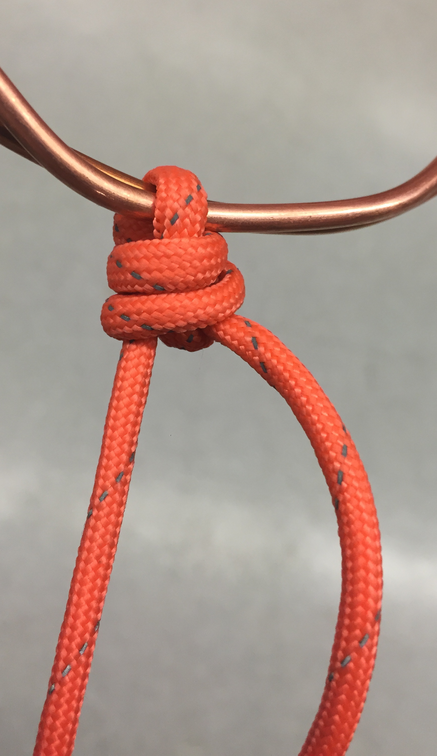
\includegraphics[width=1.4\paperwidth,height=1.4\paperheight,keepaspectratio]{title_pic.png}
\vfill
}}}

\begin{document}

\AddToShipoutPicture*{\BackgroundPic}

\begin{titlepage}
  \color{white}
  \begin{center}
    {\fontsize{50}{60}\selectfont \textbf{How to Tie a\\ \bigskip Penny Knot}}
    \vfill
    \large{
      Michael Cailotto\\
      Jacob Hladky\\
      Fiona Kelly\\
      Heriberto Rodriguez\\
      \bigskip
      California Polytechnic State University\\
      San Luis Obispo, CA\\
      \today
    }
  \end{center}
\end{titlepage}

\pagenumbering{roman}

\tableofcontents

\listoffigures
\begingroup
\let\clearpage\relax
\listoftables
\endgroup
\clearpage

\pagenumbering{arabic}

\section{Introduction}
This guide will teach you how to tie a penny knot. The penny knot is used to attach a fish hook to fishing line, and is one of the standard knots used in fishing. This guide is for beginning fishermen just starting out or for an old pro who wants to refresh his or her knot knowledge.\\\\
For beginners, we recommend learning the knot on a large scale model of a fish hook, referred to here as a ``training hook. '' The standard fishing line should be substituted with a thicker rope like parcord when using the training hook. Once you feel that you have mastered the knot with the training hook, apply your knowledge to the real thing.

\subsection{Product Description}
Completion of this guide will result in the ability to tie a penny know quickly and repeatedly, on ropes of varying thickness. This steps in this guide should be repeatedly as many times as necessary in order to obtain mastery of this knot.

\subsection{Safety Warnings}

\begin{infobox}[backgroundcolor=yellow]
  {\infosign} \textbf{ROPE BURN} --- Fishing line will be used in this guide. Ropes that move quickly can cause friction rope burns. Don't get burned!
\end{infobox}

\begin{infobox}[backgroundcolor=red, linecolor=white]
  \color{white} {\warningsign} \textbf{SHARP EDGES} --- Scissors will be used in this guide. Scissors have sharp edges! Don't cut yourself on the scissors!
\end{infobox}

\begin{infobox}[backgroundcolor=red, linecolor=white]
  \color{white} {\warningsign} \textbf{FISH HOOKS} --- Fish hooks will be used in this guide. Don't get hooked on the fish hook! It's very painful.
\end{infobox}

\subsection{Required Tools}
You can try a penny knot around any ring, but the knot is designed for fish hooks, and thus you will need:
\begin{itemize}
\item 1 x fish hook
\item 1 x fishing line
\item 1 x scissors
\end{itemize}

If you are using the training hook, then replace the fishing line with some thicker rope such as parcord.

\section{Glossary}
\subsection{Knot Terms}
\begin{itemize}
\item \textbf{BIGHT} --- A bend in the rope that forms a U-shape.
\item \textbf{OVERHAND LOOP} --- A loop in the rope where the \textbf{TAG END} goes over the \textbf{STANDING PART}
\item \textbf{STANDING END} --- The end of the rope that you are not using the form the know. The length of the rope from where the knot ends to the other end is will also be referred to as the \textbf{STANDING END} or \textbf{STANDING PART}.
\item \textbf{TAG END} --- The end of the rope that you will be using to form the knot. Also called the \textbf{WORKING END} or \textbf{RUNNING END}
\item \textbf{UNDERHAND LOOP} --- A loop in the rope where the \textbf{TAG END} goes under the \textbf{STANDING PART}

\end{itemize}

\subsection{Fishing Terms}
\begin{itemize}
\item \textbf{BEND} --- The part of the hook that forms the ``U'' shape.
\item \textbf{EYE} --- The hole at the top of the hook, where you thread the fishing line through.
\item \textbf{POINT} --- The sharp end of the hook.
\item \textbf{SHANK} --- The edge of the hook from the top of the bend to the eye.
\end{itemize}

\subsection{Rope Terms}
\begin{itemize}
\item \textbf{PARCORD} --- A thin, highly elastic kind of general-purpose rope made from nylon. Called \textbf{PARCORD} because of its historical use in the suspension lines of parachutes.
\end{itemize}

\section{Instructions}
\begin{enumerate}

\item \label{itm:hold1} Hold the hook in your left hand and the tag end of the line with your right hand.

\item \label{itm:thread} Thread about 6in of the tag end of the line through the eye of the hook

  \begin{figure}[ht!]
    \centering
    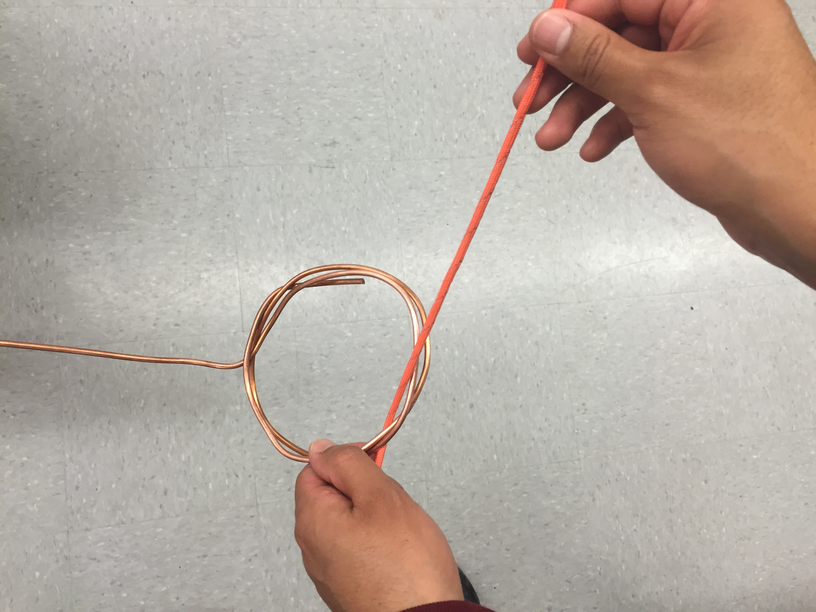
\includegraphics[width=1\textwidth]{pic0.png}
    \caption{\textit{Step~\ref{itm:hold1}} and \textit{Step~\ref{itm:thread}}. The hook with 6in of rope threaded through its eye.}
    \label{fig:pic0}
  \end{figure}

\clearpage

\item \label{itm:form} Form an overhand loop about the size of your hand with the tag end, making sure that the tag end goes over the standing end.

\begin{figure}[ht!]
    \centering
    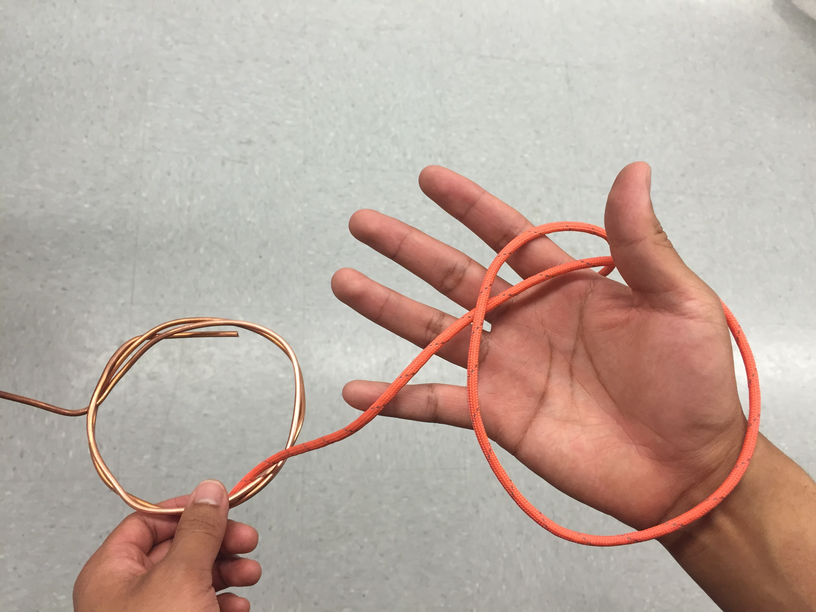
\includegraphics[width=1\textwidth]{pic1.png}
    \caption{\textit{Step~\ref{itm:form}}. An overhand loop.}
    \label{fig:pic1}
 \end{figure}

\clearpage

\item \label{itm:place} Place the loop under the standing part of the line.

\begin{figure}[ht!]
    \centering
    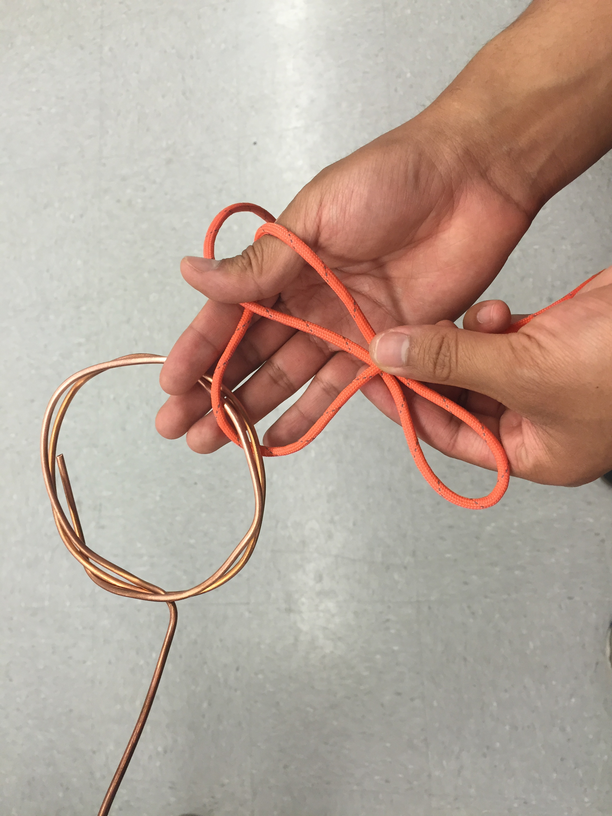
\includegraphics[width=0.9\textwidth]{pic2.png}
    \caption{\textit{Step~\ref{itm:place}}. The overhand loop.}
    \label{fig:pic2}
 \end{figure}

\clearpage

\item \label{itm:twist1} Twist the loop over the standing part of the line.

\begin{figure}[ht!]
    \centering
    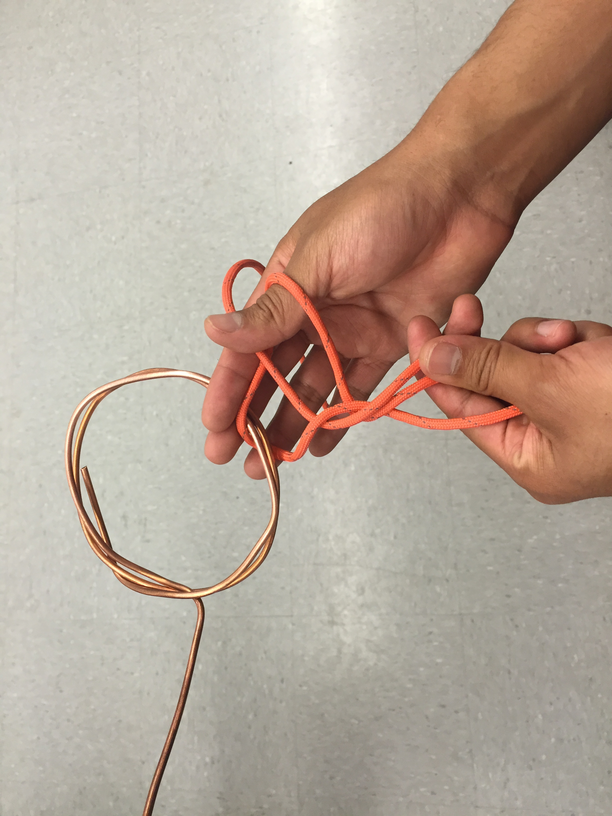
\includegraphics[width=0.9\textwidth]{pic3.png}
    \caption{\textit{Step~\ref{itm:twist1}}. Halfway through first twist.}
    \label{fig:pic3}
 \end{figure}


\begin{figure}[ht!]
  \centering
  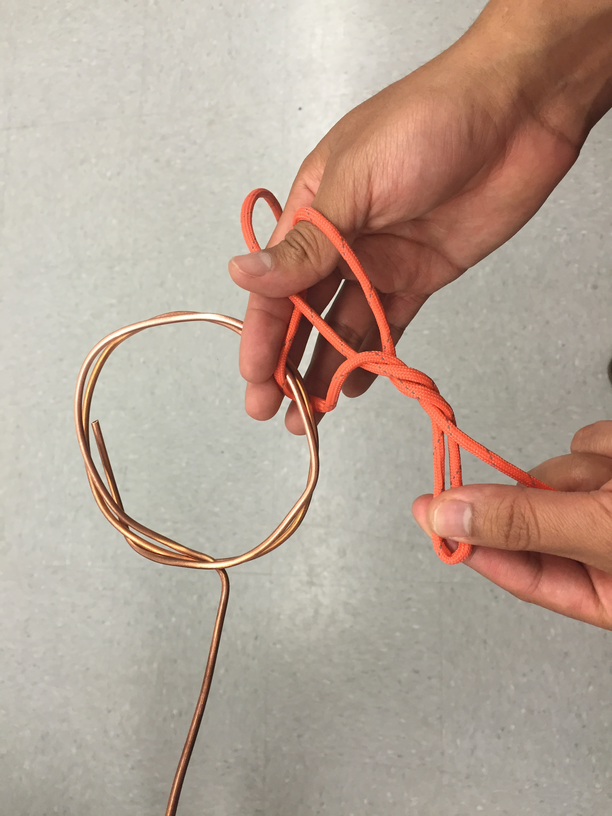
\includegraphics[width=0.9\textwidth]{pic4.png}
  \caption{\textit{Step~\ref{itm:twist1}}. Completion of the first twist.}
  \label{fig:pic4}
\end{figure}

\clearpage

\item \label{itm:twist2} Twist the loop over the standing part of the line again.

\item (Optional) Twist the loop over the standing end of the line a third time.

\begin{figure}[ht!]
    \centering
    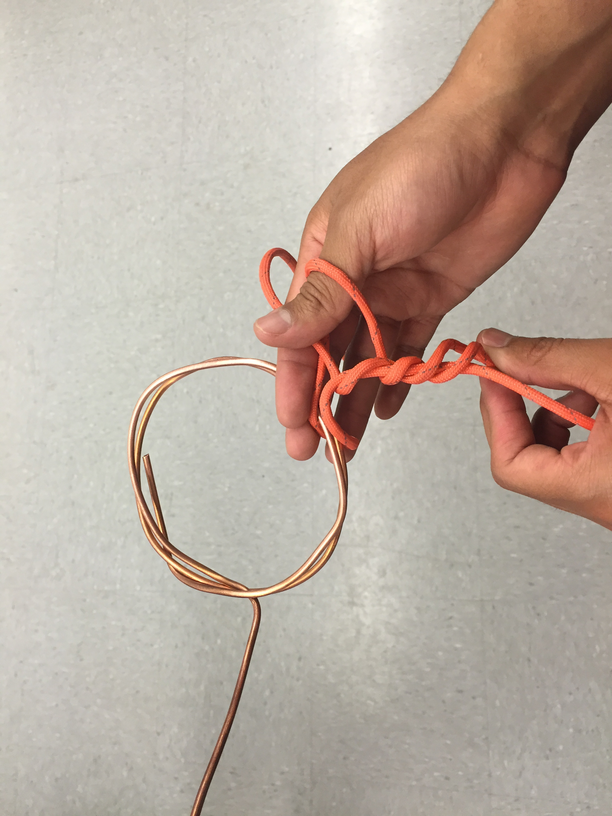
\includegraphics[width=0.9\textwidth]{pic5.png}
    \caption{\textit{Step~\ref{itm:twist2}}. The second twist.}
    \label{fig:pic5}
 \end{figure}

\clearpage

\item \label{itm:hold2} Hold the end of the loop in one hand and hold the tag end of the line in your other hand.

\begin{figure}[ht!]
    \centering
    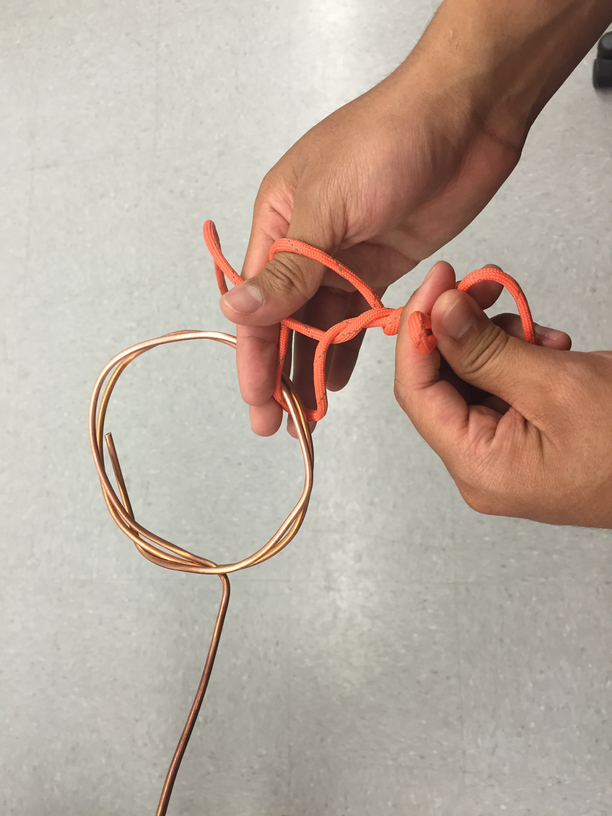
\includegraphics[width=0.9\textwidth]{pic6.png}
    \caption{\textit{Step~\ref{itm:hold2}}. Holding the twists.}
    \label{fig:pic6}
 \end{figure}

\clearpage

\item \label{itm:push} Push the tag end of the line through the loop.

\begin{figure}[ht!]
    \centering
    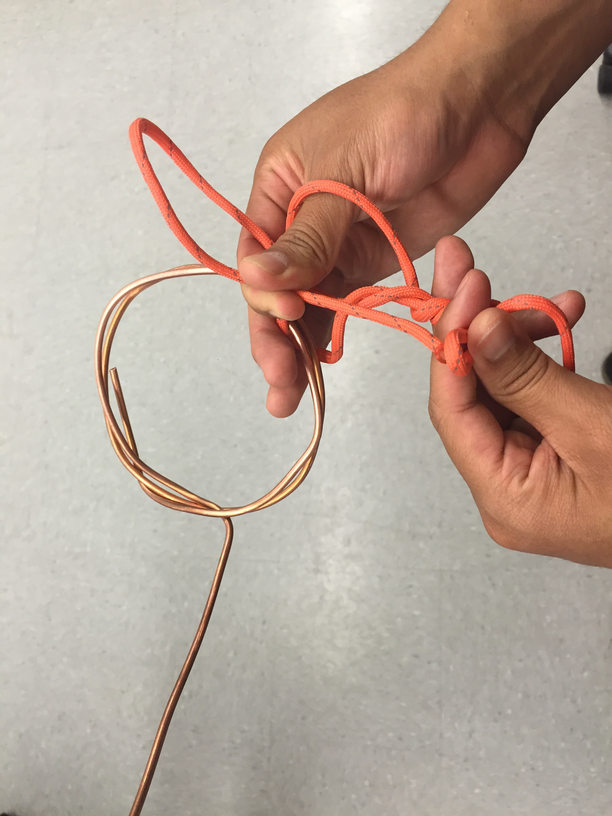
\includegraphics[width=0.9\textwidth]{pic7.png}
    \caption{\textit{Step~\ref{itm:hold2}}. The tag end and the final loop.}
    \label{fig:pic7}
 \end{figure}

\clearpage

\item \label{itm:pull} Pull on the standing end of the line until the knot is next to the eye.

\begin{figure}[ht!]
    \centering
    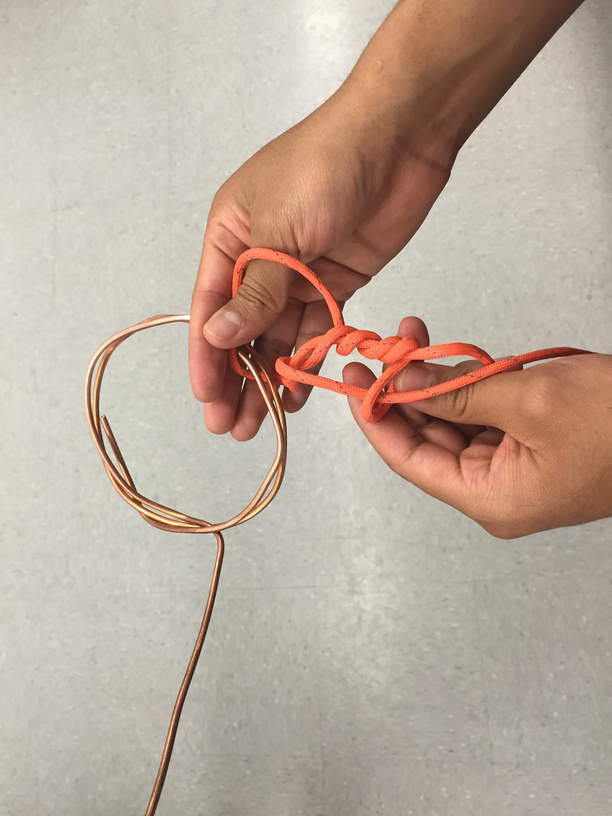
\includegraphics[width=0.9\textwidth]{pic8.png}
    \caption{\textit{Step~\ref{itm:pull}}. Pulling on the knot.}
    \label{fig:pic8}
 \end{figure}

\clearpage

\item \label{itm:tighten} Tighten and asjust the knot until the tag end is perpendicular to the knot, and the knot ``locks.''

\begin{figure}[ht!]
    \centering
    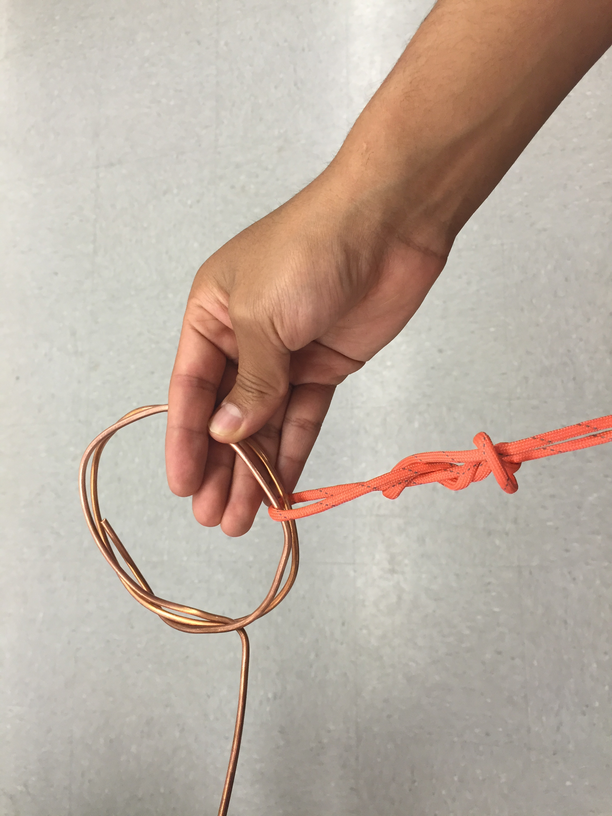
\includegraphics[width=0.9\textwidth]{pic9.png}
    \caption{\textit{Step~\ref{itm:tighten}}. Adjusting the knot.}
    \label{fig:pic9}
 \end{figure}

\begin{figure}[ht!]
    \centering
    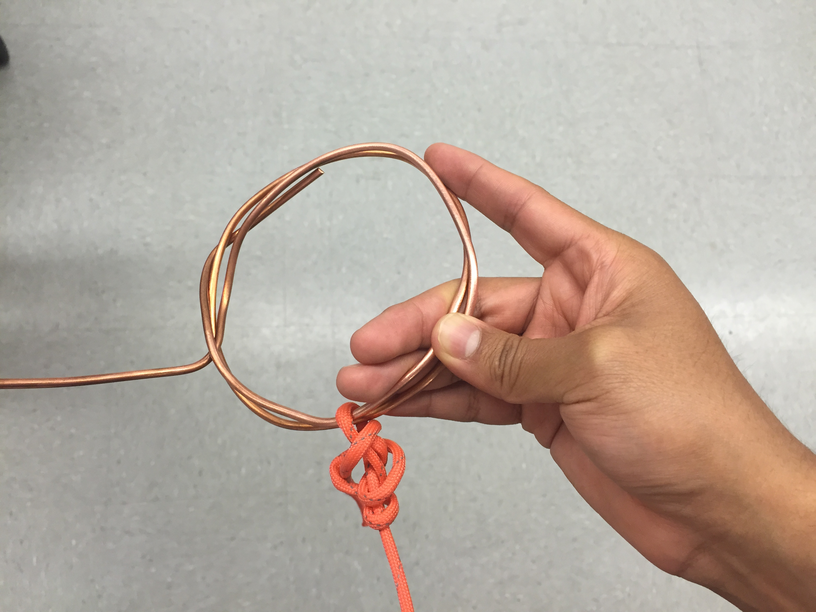
\includegraphics[width=1\textwidth]{pic10.png}
    \caption{\textit{Step~\ref{itm:tighten}}. Final adjustments.}
    \label{fig:pic10}
 \end{figure}

\begin{figure}[ht!]
    \centering
    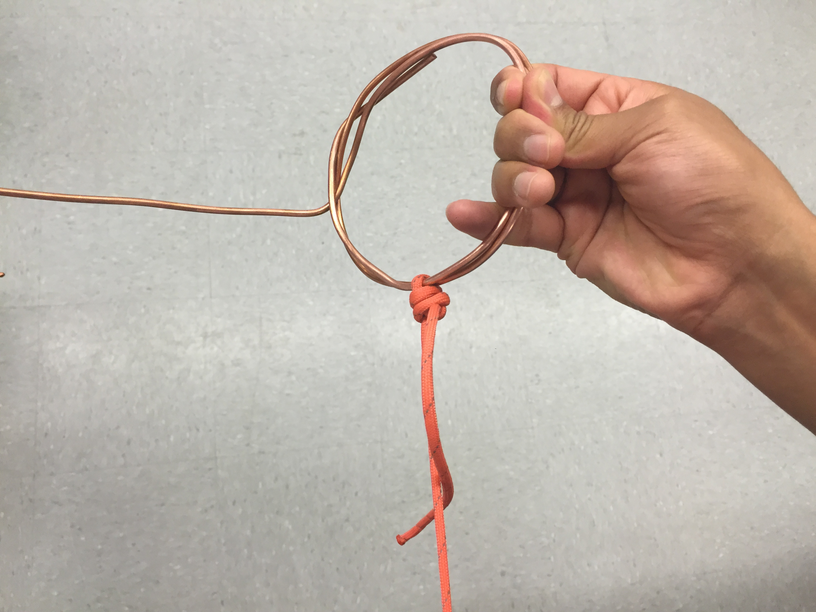
\includegraphics[width=1\textwidth]{pic11.png}
    \caption{\textit{Step~\ref{itm:tighten}}. The completed knot before the excess tag end is cut.}
    \label{fig:pic11}
 \end{figure}

\clearpage

\item \label{itm:cut} Cut the excess line from the knot. That's it! Enjoy fishing with the help of the penny knot!

\begin{figure}[ht!]
    \centering
    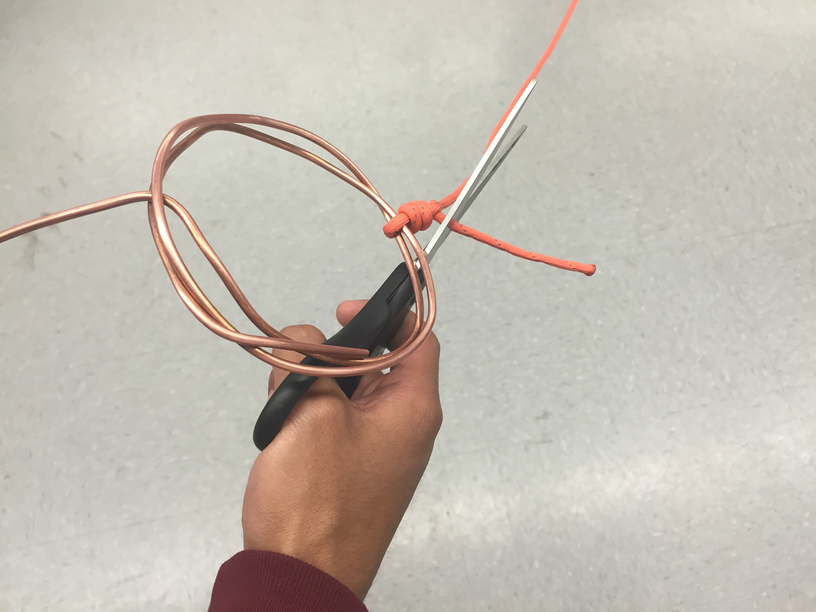
\includegraphics[width=1\textwidth]{pic13.png}
    \caption{\textit{Step~\ref{itm:cut}}. Cutting the tag end.}
    \label{fig:pic13}
 \end{figure}

\end{enumerate}

\section{Works Cited}

\textit{Not complete at this time}

\end{document}
